\chapter{Density of States}
\section{Schrodinger Equation}
Although the classical physics was well developed in 1900s, the black body radiation implicitly indicated that something is missing in the classical physics. From classical physics, the more heat putting in an object would increase the kinetic energy of the object, and thus the energy of the emitted radiation should increase with the frequency which is known as "ultraviolet catastrophe." However, this contradicted with the experimental results that the radiation intensity tends to be zero at short wavelength (higher frequency) regime. To explain this black body radiation, the (implicit) emitted energy quantization and concept of photon (particle of light) were proposed by Planck in 1900\footnote{Einstein explicitly assumed that the electromagnetic radiation is quantized in 1905.}. After that, physicists gradually noticed that every object exhibits both wave-particle duality and the energy states of a system are quantized. Finally, in 1925 Schrodinger wrote down an equation analogous to a wave equation: Schrodinger equation \begin{equation}
    i\hbar\frac{\partial \Psi}{\partial t} = -\frac{\hbar^{2}}{2m_{0}}\frac{\partial^{2}}{\partial x^{2}}\Psi + V\Psi
\end{equation} where $\Psi$ is the wavefunction of a particle, $m_{0}$ is the rest mass of the particle, and $V$ is the potential energy experienced by a particle.
\subsection{Time-Independent Schrodinger Equation}
The time independent Schrodinger equation\footnote{D. J. Griffiths, Introduction to Quantum Mechanics, Chapter 2.} predicts that the wavefunctions are able to form the standing waves which is called stationary states (also called "orbitals," such as atomic orbitals and molecular orbitals). In stationary states, the wavefunction can be divided into two parts using separation of variation method: \begin{equation}
    \Psi = \psi\left(x\right) \varphi\left(t\right)
\end{equation} where $\psi$ is a function of $x$ alone, and $\varphi$ is a function of $t$ alone. There, we can rewrite Equation (2.1) \begin{equation}
    i\hbar\psi\frac{\partial \varphi}{\partial t} = -\frac{\hbar^{2}}{2m_{0}}\frac{\partial^{2}\psi}{\partial x^{2}}\varphi + V\psi\varphi
\end{equation} Dividing through by $\psi\varphi$: \begin{equation}
    i\hbar\frac{1}{\varphi}\frac{\partial \varphi}{\partial t} = -\frac{\hbar^{2}}{2m_{0}}\frac{1}{\psi}\frac{\partial^{2}\psi}{\partial x^{2}} + V
\end{equation} Now, the left side and the right side are functions of $t$ and $x$, respectively\footnote{Here, $V$ is only a function of $x$.}. Thus, both sides are equqal to a constant $E$. Then \begin{equation}
    i\hbar\frac{1}{\varphi}\frac{\partial \varphi}{\partial t} = E
\end{equation} and \begin{equation}
    -\frac{\hbar^{2}}{2m_{0}}\frac{1}{\psi}\frac{\partial^{2}\psi}{\partial x^{2}} + V = E
\end{equation} The general solution of Equation (2.5) is \begin{equation}
    \varphi\left(t\right) = e^{-iEt/\hbar}
\end{equation} and Equation (2.6) becomes \begin{equation}
    -\frac{\hbar^{2}}{2m_{0}}\frac{\partial^{2}\psi}{\partial x^{2}} + V\psi = E\psi \nonumber
\end{equation} Or \begin{equation}
    \boxed{\left[-\frac{\hbar^{2}}{2m_{0}}\frac{\partial^{2}}{\partial x^{2}} + V\right]\psi = E\psi}
\end{equation} The Equation (2.8) is called the {\bf time-independent Schrodinger equation} and \begin{equation}
    -\frac{\hbar^{2}}{2m_{0}}\frac{\partial^{2}}{\partial x^{2}} + V \equiv H
\end{equation} is called the {\bf Hamiltonian} which is an operator. The Equation (2.8) implicitly states that solving the Schrodinger equation is an eigenvalue problem. The physical meaning of the constant $E$ is actually the energy of the particle. Thus, the energy available in a quantum system can be determined by Equation (2.8). Taking a simplest example of a free electron ($V = 0$), we can immediately solve Schrodinger equation and get \begin{equation}
    \psi = A e^{ikx}
\end{equation} and \begin{equation}
    E = \frac{\hbar^{2}k^{2}}{2m_{0}}
\end{equation} where $k$ is the wavenumber. Note that the Equation (2.10) is a plane wave solution. If we apply the periodic boundary condition, we have \begin{equation}
    \psi\left(x=0\right) = \psi\left(x=L\right)\nonumber
\end{equation} \begin{equation}
    1 = e^{ikL} \Rightarrow kL=2\pi n \Rightarrow k = \frac{2\pi}{L}n
\end{equation} and \begin{equation}
    E = \frac{\hbar^{2}}{2m_{0}}\frac{4\pi^{2}}{L^{2}}n^{2}
\end{equation} where $n$ is an integer. Thus, for an one-dimensional free electron, the density of states is \begin{align}
    D\left(E\right)&= \sum_{n}{\delta\left(E-E_{n}\right)} = \sum_{n}{\delta\left(E-\frac{\hbar^{2}}{2m_{0}}\frac{4\pi^{2}}{L^{2}}n^{2}\right)}\nonumber\\
    & = \int_{-\infty}^{\infty}\frac{dk}{\Delta k}\delta\left(E-\frac{\hbar^{2}k^{2}}{2m_{0}}\right),\quad\frac{\hbar^{2}k^{2}}{2m_{0}}\equiv z,\quad \Delta k = \frac{2\pi}{L} \nonumber\\
    & = \frac{Lm_{0}}{\pi\hbar}\frac{1}{\sqrt{2m_{0}}}\int_{0}^{\infty}dz\frac{1}{\sqrt{z}}\delta\left(E-z\right) \nonumber\\
    & = \frac{Lm_{0}}{\pi\hbar}\frac{1}{\sqrt{2m_{0}}}\frac{1}{\sqrt{E}}
\end{align} Note that the electron has up- and down-spin degeneracy, so the total DOS (per unit length per unit energy) is \begin{equation}
    \boxed{\frac{D\left(E\right)}{L} \equiv D\left(E\right) = \frac{2m_{0}}{\pi\hbar}\frac{1}{\sqrt{2m_{0}}}\frac{1}{\sqrt{E}}}
\end{equation}
\subsection{Formalism in Quantum Mechanics}
The formalism in quantum mechanics is somehow different from the classical physics. There are two important constructs: wavefunctions and operators, which represent the state of a system and observables. In mathematical language (linear algebra), the wavefunctions are vectors and, the operators are the linear transformations. A vector in an $N$-dimensional space can be expressed using a specified orthogonal basis \begin{equation}
    \big|\psi\big>\rightarrow\vec{\psi}=
    \left[
    \begin{matrix}
    \phi_{1} \\
    \phi_{2} \\
    \vdots \\
    \phi_{N} \\
    \end{matrix}
    \right]
\end{equation} and \begin{equation}
    \big<\psi\big|\rightarrow\vec{\psi}^{\dagger}=
    \left[
    \begin{matrix}
    \phi_{1}^{*} & \phi_{2}^{*} & \ldots & \phi_{N}^{*}
    \end{matrix}
    \right]
\end{equation} The Equations (2.16) and (2.17) are the ket and bra, which form the {\bf{Dirac notation}}. In general, the solution of Schrodinger equation is \begin{equation}
    \big|\psi\big>=\sum_{j}^{N}{c_{j}\big|\phi_{j}\big>}
\end{equation} and $\phi_{j}$'s form a set of orthogonal basis in $N$-dimensional {\bf Hilbert space} obeying \begin{equation}
    \int_{-\infty}^{\infty}\phi_{i}^{*}\left(x\right)\phi_{j}\left(x\right)dx =
    \begin{cases}
    1 & \text{if }i = j \\
    0 & \text{if }i \neq j
    \end{cases}
\end{equation} where $\phi_{i}^{*}$ is the complex conjugate of $\phi_{i}$ and the Equation (2.19) is the inner product of two bases. The coefficients $c_{j}$'s can be obtained by \begin{equation}
    \boxed{\big<\phi_{k}\big|\psi\big> = \int_{-\infty}^{\infty}\phi_{k}^{*}\left[c_{1}\phi_{1}+c_{2}\phi_{2}+\ldots+c_{k}\phi_{k}+\ldots\right]dx = c_{k}}
\end{equation} Using Dirac notation to rewrite Schrodinger equation, we have\footnote{The bold font represents an operator here and later on. For example, the Hamiltonian is an operator and the energy $E$ is a scalar.} \begin{equation}
    E\big|\psi\big> = \vec{H}\big|\psi\big>
\end{equation} If multiplying $\big<\phi_{k}\big|$ to the Equation (2.21), \begin{equation}
    \sum_{j}Ec_{j}\big<\phi_{k}\big|\phi_{j}\big>=\sum_{j}\big<\phi_{k}\big|\vec{H}c_{j}\big|\phi_{j}\big> \nonumber
\end{equation} \begin{equation}
    \Rightarrow Ec_{k} = \sum_{j}{\big<\phi_{k}\big|\vec{H}\big|\phi_{j}\big>c_{j}} = \sum_{j}{H_{k,j}c_{j}}
\end{equation} where \begin{equation}
    H_{k,j} \equiv \big<\phi_{k}\big|\vec{H}\big|\phi_{j}\big>
\end{equation} Thus, \begin{equation}
    E \left[
    \begin{matrix}
    c_{1} \\
    c_{2} \\
    \vdots \\
    c_{N} \\
    \end{matrix}
    \right] = \left[
    \begin{matrix}
    H_{11}c_{1}+H_{12}c_{2}+\ldots \\
    H_{21}c_{1}+H_{22}c_{2}+\ldots \\
    \vdots \\
    \end{matrix}
    \right] = \vec{H}\left[c\right] \nonumber
\end{equation} \begin{equation}
    \Rightarrow\boxed{E\left[c\right]=\vec{H}\left[c\right]}
\end{equation} The Equation (2.24) explicitly indicates that solving the Schrodinger equation is mathematically an eigenvalue problem, where $\left[c\right]$ is the eigenvectors with the corresponding eigenvalues $E$.
\subsection{Basis Transformation}
As seen in Equation (2.18), there are multiple choices of the set of basis. The question is: how can we change the basis and what are the mathematical and physical meanings of such transformation? Let's consider \begin{equation}
    \big|\psi\big>=\sum_{j}{c_{j}\big|\phi_{j}\big>}=\sum_{k}{d_{k}\big|u_{k}\big>}
\end{equation} \begin{equation}
    \Rightarrow d_{i} = \big<u_{i}\big|\psi\big> = \sum_{j}{\big<u_{i}\big|\phi_{j}\big>c_{j}} \equiv \sum_{j}{M_{ij}c_{j}}
\end{equation} \begin{equation}
    \Rightarrow \left[\begin{matrix}
    d_{1} \\
    d_{2} \\
    \vdots \\
    \end{matrix}
    \right] = \left[M\right]\left[\begin{matrix}
    c_{1} \\
    c_{2} \\
    \vdots \\
    \end{matrix}
    \right]
\end{equation} where $\vec{M}$ is the rotation matrix. Mathematically, the Equation (2.27) represents the rotation of a vector: \begin{equation}
    \vec{A}\big|x\big> = \big|y\big>
\end{equation} and \begin{equation}
    \big<y\big| = \big<x\big|\vec{A}^{\dagger}
\end{equation} such taht \begin{equation}
    \big<y\big|\vec{A}\big|x\big> = \big<y\big|y\big> \nonumber
\end{equation} \begin{equation}
    \Rightarrow \big<x\big|\vec{A}^{\dagger}\vec{A}\big|x\big> = \big<y\big|y\big> = \big<x\big|x\big> = 1
\end{equation} Therefore, \begin{equation}
    \vec{A}^{\dagger}\vec{A} = \vec{I}
\end{equation} where $\vec{I}$ is the identity matrix and the Equation (2.31) is called unitary transformation. Now if we have a two-dimensional vector \begin{equation}
    \big|r\big> = a\big|x\big> + b\big|y\big>
\end{equation} where \begin{equation}
    a = \big<x\big|r\big> \quad \text{and} \quad b = \big<y\big|r\big> \nonumber
\end{equation} then \begin{align}
    \big|r\big>& = \big|x\big>a + \big|y\big>b = \big|x\big>\big<x\big|r\big> + \big|y\big>\big<y\big|r\big>\nonumber \\
    & = \underbrace{\left(\big|x\big>\big<x\big| + \big|y\big>\big<y\big|\right)}_{=1}\big|r\big>
\end{align} More generally, \begin{equation}
    \sum_{i}{\big|\phi_{i}\big>\big<\phi_{i}\big|} = 1
\end{equation} The Equation (2.34) is called the identity operator. By using the identity operator, we obtain the new Hamiltonian in a new set of basis. \begin{align}
    H_{kj}& = \big<u_{k}\big|\vec{H}\big|u_{l}\big>\nonumber\\
    & = \sum_{i,j}{\big<u_{k}\big|\phi_{i}\big>\big<\phi_{i}\big|\vec{H}\big|\phi_{j}\big>\big<\phi_{j}\big|u_{l}\big>} \nonumber\\
    & = \sum_{i,j}{M_{ki}H_{ij}M_{jl}} \nonumber
\end{align} \begin{equation}
    \Rightarrow \vec{M}^{\dagger}\vec{H}^{\text{old}}\vec{M} = \vec{H}^{\text{new}}
\end{equation} As mentioned earlier, solving the Schrodinger equation is a eigenvalue problem. Thus, the property of the Hamiltonian should be properly explored. Suppose we have the following eigenvalue problem \begin{equation}
    \vec{A}\big|x\big> = \lambda\big|x\big> \quad \text{and} \quad \big<x\big|\vec{A}^{\dagger} = \lambda^{\dagger}\big<x\big|
\end{equation} By multiplying $\big<x\big|$ and $\big|x\big>$ from the left and right sides respectively to the Equation (2.36), we have \begin{equation}
    \big<x\big|\vec{A}\big|x\big> = \lambda \quad \text{and} \quad \big<x\big|\vec{A}^{\dagger}\big|x\big> = \lambda^{\dagger}
\end{equation} then \begin{equation}
    \big<x\big|\vec{A}\big|x\big> - \big<x\big|\vec{A}^{\dagger}\big|x\big> = \big<x\big|\vec{A}-\vec{A}^{\dagger}\big|x\big> = \lambda - \lambda^{\dagger} = 0 \quad \text{if} \quad \lambda \in \Re \nonumber
\end{equation} \begin{equation}
    \Rightarrow \vec{A} = \vec{A}^{\dagger}
\end{equation} where $\vec{A}$ is called the {\bf Hermition Matrix}. Because the energy $E$ is real, {\bf the Hamiltonian is also a Hermition matrix}. From Copenhagen interpretation of quantum mechanics, the square of the coefficient $c_{i}$ is the probability having the $i$th state and the total probability of all possible outcomes has to be one \begin{align}
    \big<\psi\big|\psi\big>& = \sum_{ij}{c_{i}^{*}\big<\phi_{i}\big|c_{j}\big|\phi_{j}\big>}\nonumber\\
    & = \sum_{ij}{c_{i}^{*}c_{j}\big<\phi_{i}\big|\phi_{j}\big>} = \sum_{i}{\big|c_{i}\big|^{2}}\nonumber\\
    & = \text{Trace}\left[\begin{matrix}
    \big|c_{1}\big|^{2} & 0 & \ldots \\
    0 & \big|c_{2}\big|^{2} & \ldots \\
    \vdots & \vdots & \ddots
    \end{matrix}
    \right] = 1
\end{align} where each element on the digonal of the matrix is the probability at such state. The momentum operator $\vec{p}$ is\footnote{D. J. Griffiths, Introduction to Quantum Mechanics, Chapter 1.} \begin{equation}
    \vec{p} = -i\hbar\frac{\partial}{\partial x}
\end{equation} Thus, the expectation value of the momentum is\footnote{$\big<x\big|\vec{p}\big|x'\big> = -i\hbar\delta'\left(x-x'\right)$. See R. Shankar, Principles of Quantum Mechanics, second edition, page 64-64.} \begin{align}
    \big<\vec{p}\big>& = \big<\psi\big|\vec{p}\big|\psi\big> = \sum_{ij}{c_{i}^{*}c_{j}\underbrace{\big<\phi_{i}\big|\vec{p}\big|\phi_{j}\big>}_{= \delta_{ij}p_{ij}}} \nonumber\\
    & = \text{Trace}\left(\rho^{\text{eigenbasis}}p^{eigenbasis}\right)
\end{align} where $\rho^{\text{eigenbasis}}$ is the eigenvalue of the density matrix\footnote{It can be interpreted as the probability of having electrons in a given state.}, which is more generally defined as \begin{equation}
    \rho = \sum_{i}{\rho_{i}\big|\phi_{i}\big>\big<\phi_{i}\big|}
\end{equation} where \begin{equation}
    \rho_{i} = \frac{n_{i}}{N} = \big|c_{i}\big|^{2} = \big|\phi_{i}\big>\big<\phi_{i}\big| \quad \text{and} \quad \sum_{i}{\rho_{i}} = 1
\end{equation} $n_{i}$ is the number of particles in the $i$th state and $N$ is the total number of particles in a system. Check consistency of density matrix: \begin{equation}
    n = \int_{-\infty}^{\infty}\frac{\gamma_{1}f_{1}+\gamma_{2}f_{2}}{\gamma_{1}+\gamma_{2}}D\left(E\right)dE
\end{equation} Assume $\gamma_{1} = \gamma_{2}$ and $f_{1} = f_{2} = f_{0}\left(E-\mu\right)$, we have\footnote{There is a confusion here. The unit of the density of states here is {\bf per unit energy}. However, in many semiconductor textbooks, the density of states is in unit of {\bf per unit volume (or area or length) per unit energy}. Thus, $n$ here is the total number of electrons (carriers) instead of density.} \begin{align}
    n& = \int_{-\infty}^{\infty}f_{0}\left(E-\mu\right)D\left(E\right)dE\nonumber\\
    & = \sum_{\varepsilon_{i}}{\int_{-\infty}^{\infty}f_{0}\left(E-\mu\right)\delta\left(E-\varepsilon_{i}\right)dE}\nonumber\\
    & = \sum_{\varepsilon_{i}}{f_{0}\left(E-\mu\right)} = \sum_{i}{n_{i}} = N\big<\psi\big|\psi\big> = N
\end{align}
\section{Bloch's Theorem}
If we want to describe the electron wavefunction in a solid, we need to consider the potential $V$ experienced by the electrons. Let's consider an one-dimensional lattice as shown in Fig. 2.1.
\begin{figure}[tbp]
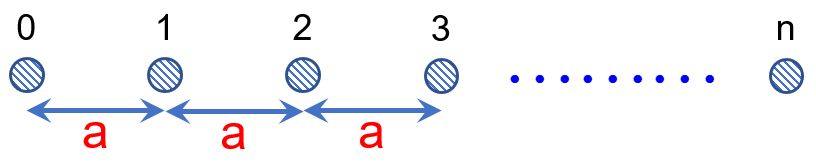
\includegraphics[width=0.7\textwidth]{figures/Fig2_1}
\centering
\caption{\small An one-dimensional lattice with lattice constant of $a$.}
\end{figure} Because there is no way to distinguish the electron wavefunction at each site, the Schrodinger equations of electrons at each site can be written as \begin{equation}
    H\big|\psi\left(\overset{\rightharpoonup}{r}+\overset{\rightharpoonup}{a}\right)\big> = E\big|\psi\left(\overset{\rightharpoonup}{r}+\overset{\rightharpoonup}{a}\right)\big>
\end{equation} \begin{equation}
    H\big|\psi\left(\overset{\rightharpoonup}{r}+2\overset{\rightharpoonup}{a}\right)\big> = E\big|\psi\left(\overset{\rightharpoonup}{r}+2\overset{\rightharpoonup}{a}\right)\big>
\end{equation} and so on. However, above equations imply infinite degeneracy in a solid which is not physical. Therefore, between each wavefunction there should be a scalar multiplier. In other words, \begin{equation}
    \big|\psi\left(\overset{\rightharpoonup}{r}+2\overset{\rightharpoonup}{a}\right)\big> = A\big|\psi\left(\overset{\rightharpoonup}{r}+\overset{\rightharpoonup}{a}\right)\big>
\end{equation} where $A$ is a scalar. Note that \begin{equation}
    \big<\psi\left(\overset{\rightharpoonup}{r}+2\overset{\rightharpoonup}{a}\right)\big|\psi\left(\overset{\rightharpoonup}{r}+2\overset{\rightharpoonup}{a}\right)\big> = A^{*}A\big<\psi\left(\overset{\rightharpoonup}{r}+\overset{\rightharpoonup}{a}\right)\big|\psi\left(\overset{\rightharpoonup}{r}+\overset{\rightharpoonup}{a}\right)\big>\nonumber
\end{equation} \begin{equation}
    \Rightarrow \big|A\big|^{2} = 1 \nonumber \Rightarrow A = e^{i\phi}
\end{equation} Thus, \begin{equation}
    \big|\psi\left(\overset{\rightharpoonup}{r}+n\overset{\rightharpoonup}{a}\right)\big> = e^{in\phi}\big|\psi\left(\overset{\rightharpoonup}{r}\right)\big> \nonumber
\end{equation} or \begin{equation}
    \boxed{\big|\psi\left(\overset{\rightharpoonup}{r}+\overset{\rightharpoonup}{L}\right)\big> = e^{i\overset{\rightharpoonup}{k}\cdot\overset{\rightharpoonup}{L}}\big|\psi\left(\overset{\rightharpoonup}{r}\right)\big>}
\end{equation} where $L (= na)$ is the length of the one-dimensional lattice and $k\left(=\frac{2\pi}{a}\right)$ is the wave number. The Equation (2.49) is called the {\bf Bloch's Theorem}. In general, the Equation (2.49) can be further expressed, for example, in three-dimensional lattice, and the relation between the wave number and the lattice size follows the Fourier transformation. \begin{equation}
    u\left(\overset{\rightharpoonup}{r}\right) = \sum_{g}{A_{g}e^{i\overset{\rightharpoonup}{g}\cdot\overset{\rightharpoonup}{r}}}
\end{equation} where the space spanned by $\overset{\rightharpoonup}{g}$ is called the {\bf reciprocal space} [see Fig. 2.2(b)], and $\overset{\rightharpoonup}{g}$ in three-dimensional lattice is \begin{align}
    \overset{\rightharpoonup}{g}& = \frac{2\pi}{a}n_{1}\hat{x} + \frac{2\pi}{b}n_{2}\hat{y} + \frac{2\pi}{c}n_{3}\hat{z}\nonumber\\
    & = n_{1}\overset{\rightharpoonup}{b_{1}} + n_{2}\overset{\rightharpoonup}{b_{2}} + n_{2}\overset{\rightharpoonup}{b_{2}}
\end{align} where $a$, $b$, and $c$ are the lattice constant of $x$, $y$, and $z$ directions, $n_{i}$'s are the integers, and $\overset{\rightharpoonup}{b_{i}}$'s are \begin{equation}
    \overset{\rightharpoonup}{b_{1}} \equiv \frac{2\pi}{a}\hat{x} \text{,} \quad \overset{\rightharpoonup}{b_{2}} \equiv \frac{2\pi}{b}\hat{y} \text{,} \quad \text{and} \quad \overset{\rightharpoonup}{b_{3}} \equiv \frac{2\pi}{c}\hat{z}
\end{equation} The Equation (2.52) can be generalized \begin{equation}
    \overset{\rightharpoonup}{b_{1}} = 2\pi\frac{\overset{\rightharpoonup}{a_{2}}\times\overset{\rightharpoonup}{a_{3}}}{\overset{\rightharpoonup}{a_{1}}\cdot\left(\overset{\rightharpoonup}{a_{2}}\times\overset{\rightharpoonup}{a_{3}}\right)}\nonumber
\end{equation} \begin{equation}
    \overset{\rightharpoonup}{b_{2}} = 2\pi\frac{\overset{\rightharpoonup}{a_{3}}\times\overset{\rightharpoonup}{a_{1}}}{\overset{\rightharpoonup}{a_{1}}\cdot\left(\overset{\rightharpoonup}{a_{2}}\times\overset{\rightharpoonup}{a_{3}}\right)}\nonumber
\end{equation} \begin{equation}
    \overset{\rightharpoonup}{b_{3}} = 2\pi\frac{\overset{\rightharpoonup}{a_{1}}\times\overset{\rightharpoonup}{a_{2}}}{\overset{\rightharpoonup}{a_{1}}\cdot\left(\overset{\rightharpoonup}{a_{2}}\times\overset{\rightharpoonup}{a_{3}}\right)}
\end{equation} where $\overset{\rightharpoonup}{a_{i}}$'s and $\overset{\rightharpoonup}{b_{i}}$'s are the basis of the real space and reciprocal space, and the denominator is the volume of the unit cell in the real space. Suppose we have a vector constructed by the basis of the real space \begin{equation}
    \overset{\rightharpoonup}{l} = ma\overset{\rightharpoonup}{a_{1}} + nb\overset{\rightharpoonup}{a_{2}} + oc\overset{\rightharpoonup}{a_{3}}
\end{equation} where $m$, $n$, and $o$ are the integers. Then, \begin{align}
    \overset{\rightharpoonup}{g}\cdot\overset{\rightharpoonup}{l}& = \left(n_{1}\overset{\rightharpoonup}{b_{1}} + n_{2}\overset{\rightharpoonup}{b_{2}} + n_{2}\overset{\rightharpoonup}{b_{2}}\right)\cdot\left(ma\overset{\rightharpoonup}{a_{1}} + nb\overset{\rightharpoonup}{a_{2}} + oc\overset{\rightharpoonup}{a_{3}}\right)\nonumber\\
    & = 2\pi\left(n_{1}m + n_{2}n + n_{3}o\right) \equiv 2\pi N
\end{align} This implies that the wavefunction will repeat after a certain translation. If we define $\overset{\rightharpoonup}{k} = \overset{\rightharpoonup}{k'} + \overset{\rightharpoonup}{g}$, the Equation (2.49) becomes \begin{align}
    \psi\left(\overset{\rightharpoonup}{r}+\overset{\rightharpoonup}{L}\right)& = e^{i\overset{\rightharpoonup}{k}\cdot\overset{\rightharpoonup}{L}}\psi\left(\overset{\rightharpoonup}{r}\right) = e^{i\left(\overset{\rightharpoonup}{k'}+\overset{\rightharpoonup}{g}\right)\cdot\overset{\rightharpoonup}{L}}\psi\left(\overset{\rightharpoonup}{r}\right)\nonumber\\
    & = \underbrace{e^{i(2\pi)N}}_{=1}e^{i\overset{\rightharpoonup}{k'}\cdot\overset{\rightharpoonup}{L}}\psi\left(\overset{\rightharpoonup}{r}\right)
\end{align} Since there is no way to distinguish $k$ and $k'$, the wavefunction will repeat after shift $k$ by $2\pi/a$. Within the region where the wavefunction does not repeat, it is called the {\bf Brillouin zone} as shown in Fig. 2.2(a).
\begin{figure}[tbp]
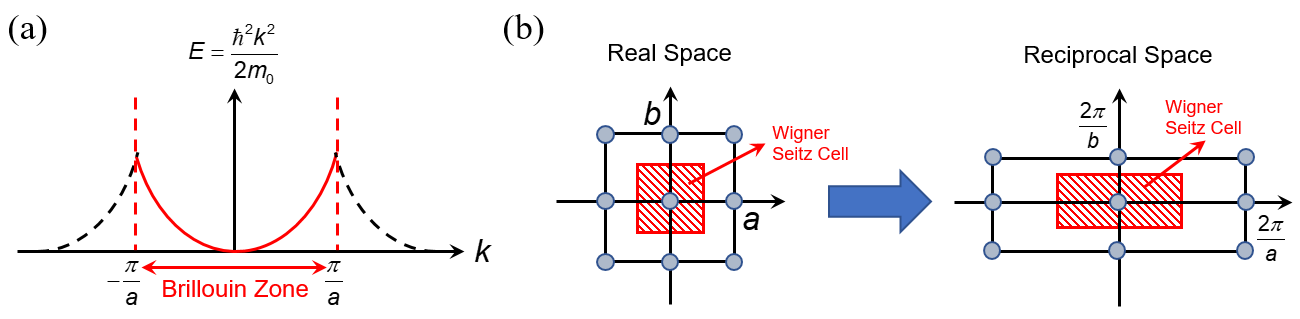
\includegraphics[width=\textwidth]{figures/Fig2_2}
\centering
\caption{\small (a) Dispersion relation ($E-k$) of an one-dimensional lattice. (b) An two-dimensional lattice in real space and reciprocal space.}
\end{figure} A common used method to obtain the Brillouin zone is to draw the {\bf Wigner Seitz cell} which bisects each nearest neighbor as shown in Fig. 2.2(b).
\section{Band Structure}
\subsection{One-Dimensional Monatomic Lattice}
Suppose we have an one-dimensional lattice shown in Fig. 2.1 and assume that the overlap of wavefunctions only presents between nearest neighbor atoms. The elements in Hamiltonian matrix are \begin{equation}
    H_{ii} = \big<\psi_{i}\big|\vec{H}\big|\psi_{i}\big> = t_{0}
\end{equation} \begin{equation}
    H_{i(i\pm 1)} = \big<\psi_{i}\big|\vec{H}\big|\psi_{i(i\pm 1)}\big> = t_{1}
\end{equation} The full matrix looks like \begin{equation}
    \vec{H} = \left[\begin{matrix}
    t_{0} & t_{1} & 0 & 0 & 0 & \ldots \\
    t_{1}^{*} & t_{0} & t_{1} & 0 & 0 & \ldots \\
    0 & t_{1}^{*} & t_{0} & t_{1} & 0 & \ldots \\
    \vdots & \vdots & \vdots & \vdots & \vdots & \ddots
    \end{matrix}
    \right]
\end{equation} The Schrodinger equation becomes\footnote{Each $\psi$ represents the wavefunction of an electron at each lattice site instead of the basis function.} \begin{equation}
    \vec{H}\vec{\psi} = \left[\begin{matrix}
    t_{0} & t_{1} & 0 & 0 & 0 & \ldots \\
    t_{1}^{*} & t_{0} & t_{1} & 0 & 0 & \ldots \\
    0 & t_{1}^{*} & t_{0} & t_{1} & 0 & \ldots \\
    \vdots & \vdots & \vdots & \vdots & \vdots & \ddots
    \end{matrix}
    \right] \left[ \begin{matrix}
    \psi_{1} \\
    \psi_{2} \\
    \psi_{3} \\
    \vdots
    \end{matrix}
    \right] = E\left[ \begin{matrix}
    \psi_{1} \\
    \psi_{2} \\
    \psi_{3} \\
    \vdots
    \end{matrix}
    \right]
\end{equation} At the $n$th row: \begin{equation}
    t_{0}\psi_{n} + t_{1}\psi_{n+1} + t_{1}^{*}\psi_{n-1} = E\psi_{n}
\end{equation} and from Block's theorem \begin{equation}
    \psi_{n} = \psi_{0}e^{ikna}
\end{equation} Thus, we have \begin{equation}
    E = t_{0} + t_{1}e^{ika} + t_{1}^{*}e^{-ika} \xrightarrow{\text{if } t_{1} \text{ is real}} t_{0} + 2t_{1}\cos{ka}
\end{equation} If $ka \ll 1$ and $t_{1} < 0$, the Equation (2.63) can be expanded by using Taylor series. \begin{align}
    E& \simeq t_{0} + 2t_{1}\left[1-\frac{\left(ka\right)^2}{2}+\ldots\right]\nonumber\\
    & = t_{0} + 2t_{1} - \left(t_{1}a^{2}\right)k^{2}\nonumber\\
    & = t_{0} - 2\big|t_{1}\big| + \left(\big|t_{1}\big|a^{2}\right)k^{2}
\end{align} Define the effective mass $m^{*}$ \begin{equation}
    m^{*} = \frac{\hbar^{2}}{2a^{2}\big|t_{1}\big|}
\end{equation} The Equation (2.64) becomes \begin{equation}
    E = E' + \frac{\hbar^{2}}{2m^{*}}k^{2}
\end{equation} where $E'\equiv t_{0}-2\big|t_{1}\big|$. When $\big|t_{1}\big|$ is large, the coupling between the nearest neighbor is strong so that the electron is "de-localized\footnote{The electron can move freely through the lattice sites.}." The effective mass approximation is usually valid for the transport phenomenon in the commonly used semiconductors since the electrons involving the transport are near the bottom of the band (within 1eV). However, when solving the binding strength between the nearest neighbors, this approximation may not be good.
\subsection{One-Dimensional Diatomic Lattice}
The diatomic lattice contains two atoms in a lattice site as shown in Fig. 2.3.
\begin{figure}[tbp]
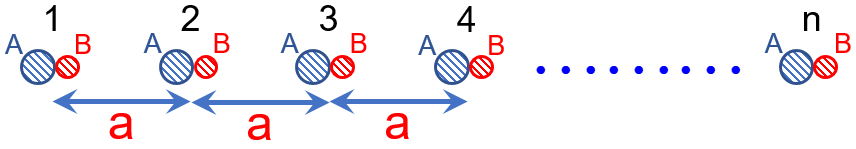
\includegraphics[width=0.7\textwidth]{figures/Fig2_3}
\centering
\caption{\small An one-dimensional diatomic (A and B) lattice with lattice constant of $a$.}
\end{figure} We assume that the wavefunction overlap only happens between the nearest neighbor atoms and atoms on site, i.e., $A_{1}$ and $B_{1}$ or $B_{1}$ and $A_{2}$. Based on this assumption, the Hamiltonian can be expressed as\\
\begin{center}
\begin{tabular}[c]{cc|cc|cc|cc|c}
     &   & 1 & 1 & 2 & 2 & 3 & 3 &  \\
     &   & A & B & A & B & A & B &  \\
     \hline
   1 & A & $t_{0}$ & $t_{1}$ & 0 & 0 & 0 & 0 & \ldots \\
   1 & B & $t_{1}^{*}$ & $t_{0}$ & $t_{2}$ & 0 & 0 & 0 & \ldots \\
     \hline
   2 & A & 0 & $t_{2}^{*}$ & $t_{0}$ & $t_{1}$ & 0 & 0 & \ldots \\
   2 & B & 0 & 0 & $t_{1}^{*}$ & $t_{0}$ & $t_{2}$ & 0 & \ldots \\
     \hline
   3 & A & 0 & 0 & 0 & $t_{2}^{*}$ & $t_{0}$ & $t_{1}$ & \ldots \\
   3 & B & 0 & 0 & 0 & 0 & $t_{1}^{*}$ & $t_{0}$ & \ldots \\
     \hline
     & & \vdots & \vdots & \vdots & \vdots & \vdots & \vdots & $\ddots$ \\
\end{tabular}
\end{center}
At the $n$th row\footnote{Each row represents each lattice site.}, the Schrodinger equation gives \begin{equation}
    \left[H\right]_{n,n}\left[\psi_{0}\right]e^{ikna} + \left[H\right]_{n,n+1}\left[\psi_{0}\right]e^{ikna}e^{ika} + \left[H\right]_{n,n-1}\left[\psi_{0}\right]e^{ikna}e^{-ika} = E\left[\psi_{0}\right]e^{ikna}
\end{equation} \begin{equation}
    \Rightarrow \left[\begin{matrix}
    t_{0} & t_{1}+t_{2}e^{ika} \\
    t_{1}^{*}+t_{2}^{*}e^{-ika} & t_{0}
    \end{matrix}
    \right] \left[\begin{matrix}
    \psi_{0A} \\
    \psi_{0B}
    \end{matrix}
    \right] = E\left[\begin{matrix}
    \psi_{0A} \\
    \psi_{0B}
    \end{matrix}
    \right]\nonumber
\end{equation} \begin{equation}
    \Rightarrow E = t_{0} \pm \sqrt{\big|t_{1}\big|^{2}+\big|t_{2}\big|^{2}+2\text{Re}\left(t_{1}t_{2}e^{ika}\right)}
\end{equation} The Equation (2.68) indicates that there are two bands in this system. If considering more interactions between more basis functions, more bands would be obtained. More generally, the Equation (2.67) can be expressed as \begin{equation}
    \sum_{m}{\left[H\right]_{n} + \left[H\right]_{n,m}e^{i\overset{\rightharpoonup}{k}\cdot\left(\overset{\rightharpoonup}{r_{m}}-\overset{\rightharpoonup}{r}\right)}}
\end{equation} where the first and second terms are the Hamiltonian matrix on the lattice site and the Hamiltonian of the overlap between the nearest neighbors respectively, and $m$ represents the nearest neighbor. The first term also can be absorbed into the second term and the Equation (2.69) becomes \begin{equation}
    \boxed{
    \sum_{m}{\left[H\right]_{n,m}e^{i\overset{\rightharpoonup}{k}\cdot\left(\overset{\rightharpoonup}{r_{m}}-\overset{\rightharpoonup}{r}\right)}} \equiv \left[h(\overset{\rightharpoonup}{k})\right]
    }
\end{equation} which is the {\bf Fourier transformation} between the reciprocal and real spaces.
\subsection{Graphene}
Graphene consists of carbon atoms with two-dimensional hexagonal lattice as shown in Fig. 2.4.
\begin{figure}[tbp]
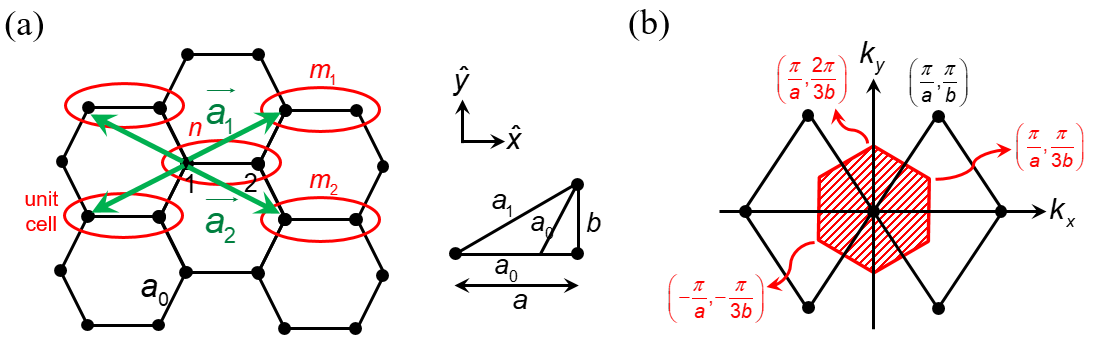
\includegraphics[width=\textwidth]{figures/Fig2_4}
\centering
\caption{\small Graphene in (a) real space (lattice constant is $a_{0}$) and (b) reciprocal space. The green arrows in (a) are the translation vectors ($\overset{\rightharpoonup}{a_{1}}$ and $\overset{\rightharpoonup}{a_{2}}$) and two atoms circled by the red line form the unit cell. The red hexagon is the Wigner Seitz cell (Brillouin zone).}
\end{figure} The coordinate of graphene in real space is defined in Fig. 2.4(a). Thus, the translation vectors in real space are \begin{equation}
    \overset{\rightharpoonup}{a_{1}} = a\hat{x} + b\hat{y}
\end{equation} \begin{equation}
    \overset{\rightharpoonup}{a_{2}} = a\hat{x} - b\hat{y}
\end{equation} \begin{equation}
    \overset{\rightharpoonup}{a_{3}} = \hat{z}
\end{equation} and \begin{equation}
    a = a_{0} + a_{0}\sin{\frac{\pi}{6}} = \frac{3a_{0}}{2}
\end{equation} \begin{equation}
    b = a_{0}\cos{\frac{\pi}{6}} = \frac{\sqrt{3}}{2}a_{0}
\end{equation} Then, the translation vectors in reciprocal space are \begin{equation}
    \overset{\rightharpoonup}{b_{1}} = 2\pi\frac{\overset{\rightharpoonup}{a_{2}}\times\overset{\rightharpoonup}{a_{3}}}{\overset{\rightharpoonup}{a_{1}}\cdot\overset{\rightharpoonup}{a_{2}}\times\overset{\rightharpoonup}{a_{3}}} = \frac{\pi}{a}\hat{x} + \frac{\pi}{b}\hat{y}
\end{equation} \begin{equation}
    \overset{\rightharpoonup}{b_{2}} = \frac{\pi}{a}\hat{x} - \frac{\pi}{b}\hat{y}
\end{equation} Due to weaker coupling of $p_{z}$ orbitals between nearest neighbors than that of $p_{x,y}$, the energy split is smaller (the energy states are closer to the Fermi level) so that the wavefunction overlap of $p_{z}$ orbitals is considered. We also assume that only the wavefunction overlap of the nearest neighbors does matter. Thus, the Hamiltonian matrix of the $n$th unit cell [see Fig. 2.4(a)] can be expressed using the Equation (2.70) \begin{equation}
    \left[H\right]_{n,n} + \left[H\right]_{n,m_{1}}e^{i\overset{\rightharpoonup}{k}\cdot\overset{\rightharpoonup}{a_{1}}} + \left[H\right]_{n,m_{2}}e^{i\overset{\rightharpoonup}{k}\cdot\overset{\rightharpoonup}{a_{2}}} + \left[H\right]_{n,m_{1}}e^{-i\overset{\rightharpoonup}{k}\cdot\overset{\rightharpoonup}{a_{1}}} + \left[H\right]_{n,m_{2}}e^{-i\overset{\rightharpoonup}{k}\cdot\overset{\rightharpoonup}{a_{2}}}
\end{equation} where \begin{equation}
    \left[H\right]_{n,n} = \left[ \begin{matrix}
    t_{0} & t \\
    t & t_{0}
    \end{matrix}
    \right],\quad
    \left[H\right]_{n,m_{1}} = \left[ \begin{matrix}
    0 & 0 \\
    t & 0
    \end{matrix}
    \right],\quad
    \left[H\right]_{n,m_{2}} = \left[ \begin{matrix}
    0 & 0 \\
    t & 0
    \end{matrix}
    \right]
\end{equation} and \begin{equation}
    t_{0} = \big<\psi_{1}\big|\vec{H}\big|\psi_{1}\big>,\quad t = \big<\psi_{1}\big|\vec{H}\big|\psi_{2}\big>,\quad t = t^{*}
\end{equation} Here, $\psi_{1,2}$ are the wavefunctions at the first (left side) and the second (right side) lattice sites in an unit cell. Therefore, the Equation (2.78) is \begin{align}
    \left[h(\overset{\rightharpoonup}{k})\right]& = \left[\begin{matrix}
    t_{0} & t + te^{-i\overset{\rightharpoonup}{k}\cdot\overset{\rightharpoonup}{a_{1}}} + te^{-i\overset{\rightharpoonup}{k}\cdot\overset{\rightharpoonup}{a_{2}}} \\
    t + te^{i\overset{\rightharpoonup}{k}\cdot\overset{\rightharpoonup}{a_{1}}} + te^{i\overset{\rightharpoonup}{k}\cdot\overset{\rightharpoonup}{a_{2}}} & t_{0}
    \end{matrix}
    \right]\equiv \left[\begin{matrix}
    t_{0} & p^{*}(\overset{\rightharpoonup}{k}) \\
    p(\overset{\rightharpoonup}{k}) & t_{0}
    \end{matrix}
    \right]
\end{align} where \begin{align}
    p(\overset{\rightharpoonup}{k})& = t + te^{i\overset{\rightharpoonup}{k}\cdot\overset{\rightharpoonup}{a_{1}}} + te^{i\overset{\rightharpoonup}{k}\cdot\overset{\rightharpoonup}{a_{2}}} = t\left[1+2e^{ik_{x}a}\cos{k_{y}b}\right]
\end{align} The eigenvalue (energy) of the matrix (2.81) is \begin{align}
    E(\overset{\rightharpoonup}{k})& = t_{0} \pm \big|p(\overset{\rightharpoonup}{k})\big|\nonumber\\
    & = t_{0} \pm t\sqrt{1+4\cos^{2}{k_{y}b}+4\cos{k_{x}a}\cos{k_{y}b}}
\end{align} The above equation describes the dispersion relationship ($E$-$k$ diagram) of graphene. Let's now consider $k_{x} = 0$: \begin{equation}
    E = t_{0} \pm t\left(1+2\cos{k_{y}b}\right)
\end{equation} If $t_{0} = 0$ is chosen, the $E$-$k_y$ plot is shown in Fig 2.5.
\begin{figure}[tbp]
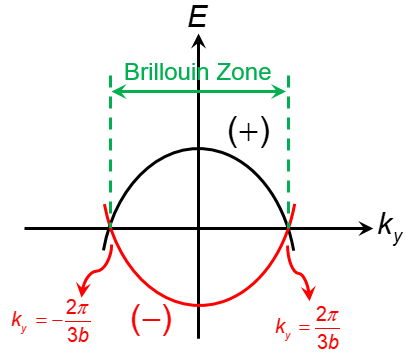
\includegraphics[width=0.4\textwidth]{figures/Fig2_5}
\centering
\caption{\small $E$-$k$ diagram of graphene at $k_{x} = 0$.}
\end{figure} Note that $k_{y} = \pm \frac{2\pi}{3b}$ are the points located at the Brillouin zone boundary as shown in Fig. 2.4(b). These points are called "Dirac points." If $k_{x} \neq 0$, the $E$-$k$ would look like a cone and the $k_{x}$ and $k_{y}$ satisfying $E = 0$ are $\left(\pm\frac{\pi}{a},\pm\frac{\pi}{3b}\right)$ where are at the zone boundary. Because the two bands are crossing at the Dirac points, the graphene behaves like a metal and the number of electrons near the Fermi level ($E_{F} = 0$) is $2\times 2\times 2 = 8$\footnote{2's are coming from two bands, up- and down-spin, and equivalent corner in the Brillouin zone.}. Now, let's consider $E$ near the Dirac point. The Taylor expansion of the Equation (2.83) assuming $t_{0} = 0$ is \begin{align}
    E(\overset{\rightharpoonup}{k})& = \pm \big|p(\overset{\rightharpoonup}{k})\big|\nonumber\\
    & \approx \pm\big|\frac{\partial p}{\partial k_{x}}\big|_{0,\pm \frac{2\pi}{3b}}\left(k_{x}-0\right) + \frac{\partial p}{\partial k_{y}}\big|_{0,\pm \frac{2\pi}{3b}}\left(k_{y}\pm\frac{2\pi}{3b}\right)\big|\nonumber\\
    & = \pm\big|-\frac{3}{2}a_{0}t\left[ik_{x}+\left(k_{y}\mp\frac{2\pi}{3b}\right)\right]\big|\nonumber\\
    & = \pm \frac{3}{2}a_{0}t\sqrt{k_{x}^{2}+\left(k_{y}\mp\frac{2\pi}{3b}\right)^{2}}\\
    & = \pm at\big|k\big| \quad \text{(linear dispersion relationship)}\nonumber
\end{align} which is different from the square dependence of $k$ for the free electron. The definition of the effective mass $m^{*} = \frac{\hbar^{2}}{\frac{\partial^{2} E}{\partial k^{2}}}$ at the Dirac points becomes physically meaningless where defining $p = \hbar k$ would be better. Since $p = 0$ at the Dirac points, there will be no current flow at that points. Around the Dirac point, the electron group velocity is \begin{equation}
    v = \frac{\partial \omega}{\partial k} = \frac{1}{\hbar}\frac{\partial E}{\partial k}=\frac{3}{2}\frac{a_{0}t}{\hbar}=\text{constant}
\end{equation} where $v$ is always written as $v_{F}$ (Fermi velocity). Thus, the E-k relation of graphene also can be written in terms of $v_{F}$ \begin{equation}
    E=\pm\hbar v_{F}\big|k\big|
\end{equation} where the electron behaves like a relativistic particle and cannot be accelerated.
\subsection{Graphene Nanotube}
Since the graphene behaves like a metal, engineering graphene to be semiconductor would be very important. One way to achieve that is to roll it into a tube as shown in Fig. 2.6.
\begin{figure}[tbp]
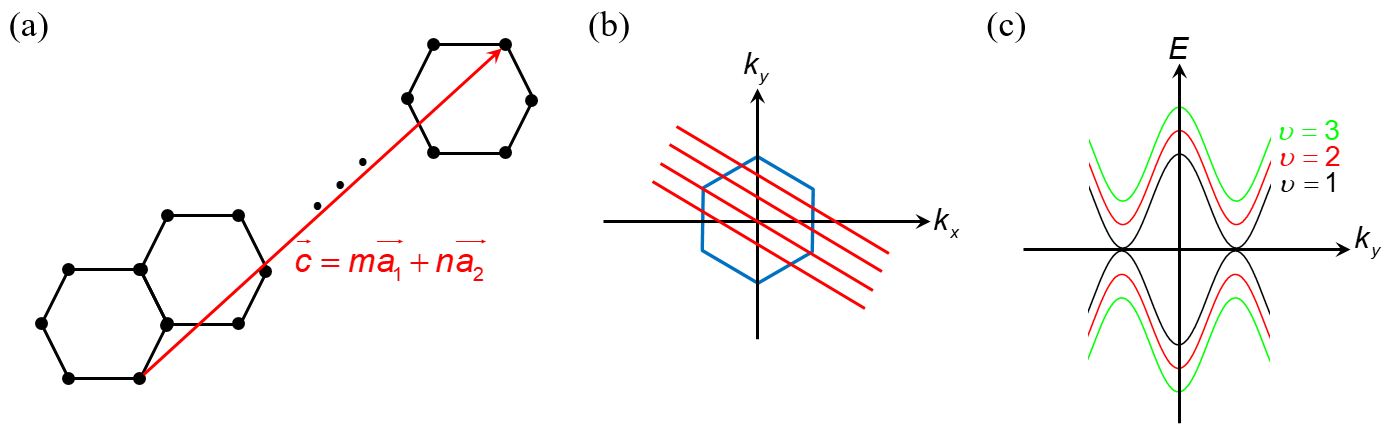
\includegraphics[width=\textwidth]{figures/Fig2_6}
\centering
\caption{\small (a) Graphene with rolling vector $\overset{\rightharpoonup}{c}$. (b) Brillouin zone of graphene and possible solutions (red straight lines) of nanotube. (c) $E-k$ diagram of graphene nanotube, assuming $k_{x}=0$.}
\end{figure} After rolling the graphene, we impose additional restriction to the lattice \begin{equation}
    \overset{\rightharpoonup}{k}\cdot\overset{\rightharpoonup}{c} = 2\pi\nu,\quad \nu\in Z
\end{equation} because the wavefunction will be a periodic function. The Equation (2.88) can be further written as \begin{equation}
    k_{y} = \frac{2\pi}{\left(m-n\right)b}\nu-\frac{\left(m+n\right)a}{\left(m-n\right)b}k_{x}
\end{equation} which represents straight lines shown in Fig. 2.6(b) depending on $\nu$ if $m$ and $n$ are known. Because the corners of the Brillouin zone [see Fig. 2.6(b)] correspond to the Dirac points, the graphene nanotube exhibits the metallic nature if the straight line crosses the corners. Therefore, whether the graphene nanotube behaves like a metal or a semiconductor would depend on how it is rolled (various combinations of $m$ and $n$).
\subsubsection{Armchair Graphene Nanotube}
If the graphene is rolled only in $x$-direction, it's called armchair nanotube as shown in Fig. 2.7.
\begin{figure}[tbp]
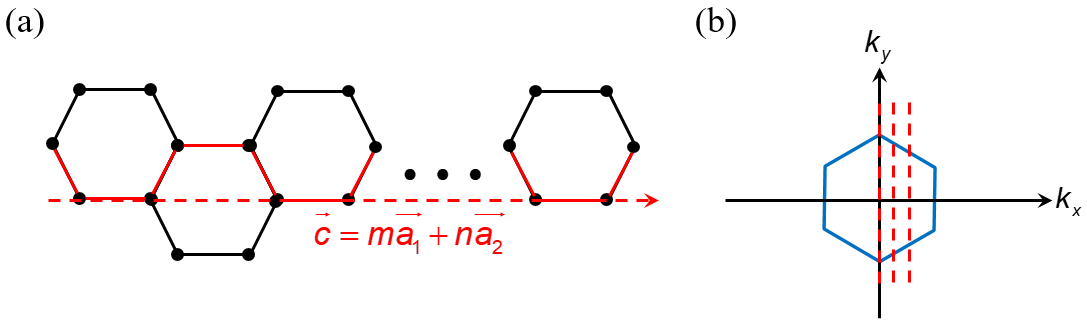
\includegraphics[width=0.9\textwidth]{figures/Fig2_7}
\centering
\caption{\small (a) Illustration of rolling an armchair nanotube. (b) Brillouin zone and possible solutions (straight lines) of armchair nanotube.}
\end{figure} Because now the wavefunction is restricted in $x$-direction, the $k_{y}$ is zero and thus the Equation (2.89) becomes \begin{equation}
    k_{x} = \frac{2\pi}{\left(m+n\right)a}\nu
\end{equation} Since $k_{x} = 0$ is a valid solution, the armchair nanotube is always metallic.
\subsubsection{Zigzag Graphene Nanotube}
If the graphene is rolled only in $y$-direction, it's called zigzag nanotube as shown in Fig. 2.8.
\begin{figure}[tbp]
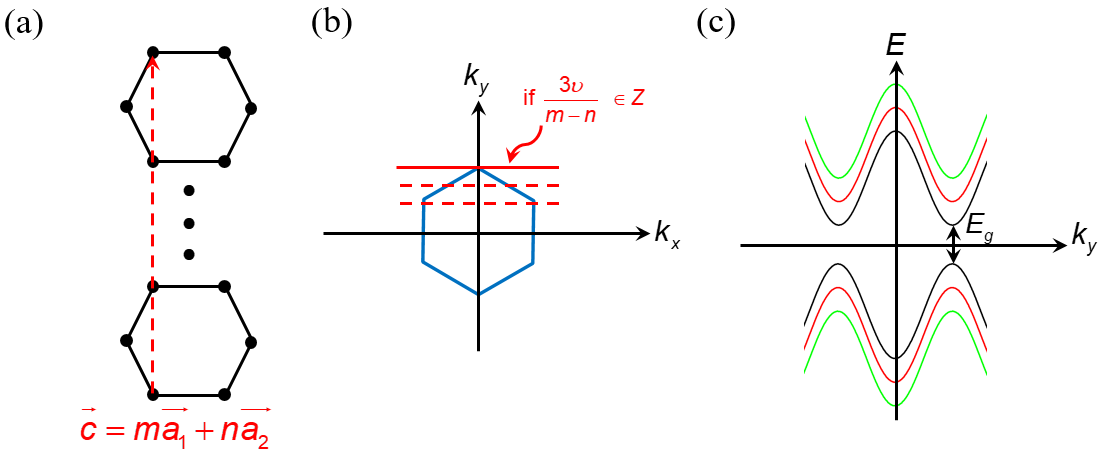
\includegraphics[width=0.9\textwidth]{figures/Fig2_8}
\centering
\caption{\small (a) Illustration of rolling a zigzag nanotube. (b) Brillouin zone and possible solutions (straight lines) of zigzag nanotube. (c) $E-k_{y}$ diagram when $(m-n)$ is not an integer multiple of 3.}
\end{figure} Because now the wavefunction is restricted in $y$-direction, the $k_{x}$ is zero and thus the Equation (2.89) becomes \begin{equation}
    k_{y} = \frac{2\pi}{3b}\frac{3\nu}{m-n}
\end{equation} If $\frac{3\nu}{m-n}$ is an integer, the zigzag nanotube will become metallic since $k_{y}$ crosses the corner of Brillouin zone [see Fig. 2.8(b)]. If $\frac{3\nu}{m-n}$ is not an integer, the zigzag nanotube behaves like a semiconductor and there is a bandgap $E_{g}$ as shown in Fig. 2.8(c). The bandgap can be evaluated using the Equation (2.85) \begin{align}
    E_{g}& = 2\times\frac{3}{2}a_{0}t\sqrt{k_{x}^{2}+\left(k_{y}\mp\frac{2\pi}{3b}\right)^{2}}\big|_{k_{x}=0,k_{y}=\frac{2\pi}{3b}\frac{3\nu}{m-n}}\nonumber\\
    & = 3a_{0}t\frac{3}{m-n}\left(\nu\mp\frac{m-n}{3}\right)\frac{2\pi}{3b}\nonumber\\
    &\xrightarrow{minimum} 3a_{0}t\frac{3}{m-n}\frac{1}{3}\frac{2\pi}{3b} = \frac{2a_{0}t\pi}{\left(m-n\right)b}
\end{align} If the diameter of the zigzag nanotube is $d$, the bandgap is \begin{equation}
    E_{g} = \frac{2a_{0}t}{d} = \frac{0.8}{d\text{ (nm)}}\text{ eV}
\end{equation} where $\pi d = (m-n)b$. The Equation (2.93) is validated by the experimental results. However, if $d<1$ nm, it is not accurate (but the trend is still correct) due to the presence of strain.
